\chapter{Introduction}
\label{introduction}
 % start numberings at 0 because (computer) science
\setcounter{figure}{-1}
\setcounter{table}{-1}
\setcounter{section}{-1}

\setlength\parindent{0pt}

\section{A Brief History of Genomics}

\begin{comment}
    describe some of the major developments over time and what that meant for cancer research in particular

    Sources / outline:
    - From Human genome to cancer genome: the first decade. [@wheeler2013human]
    - U.S. declaration of war on cancer 1971 \url{https://en.wikipedia.org/wiki/War_on_Cancer}
    - Sequencing human genome 1990-2003, time line: \url{http://web.ornl.gov/sci/techresources/Human_Genome/project/timeline.shtml}
    - WES – large scale [@wood2007genomic] → confirmed known oncogenes
    - WGS – large SVs
    - augment with cDNA sequencing (RNASeq) → gene expression, splicing, fusions, ..
    - augment with epigenetics (chromatin modification)

    - some cancers can be cured, but rarely after metastases
    - treatment vs prevention
\end{comment}

In 1990, the Human Genome Project \cite{olson1993human} set out to sequence the entire 3.2-billion-basepair-long human genome, an effort culminating in 2003 with the publication of the first human \textit{reference genome} \cite{international2004finishing}. Not only did this provide invaluable insights into human genetics, but it also paved the way for the next era in genetic research; something which would completely transform the field of genetic research. Over the next several years, massively parallel sequencers were developed by companies like Roche454 and Illumina, dramatically cutting the cost and time required to sequence a human genome, and for the first time demonstrated it's potential utility in clinical and diagnostic settings. Through sustained technological advancements over the following years, these costs have continued to decrease at exponential rates -outstripping even the pace predicted by Moore's law (Fig. \ref{fig:seqcost}) - and the long dreamed-about \textit{\$1,000 dollar genome} \cite{thousanddollargenome} \cite{sequencingcostsNHGRI} has now become a reality.

\begin{figure}[h!]
    \centering
    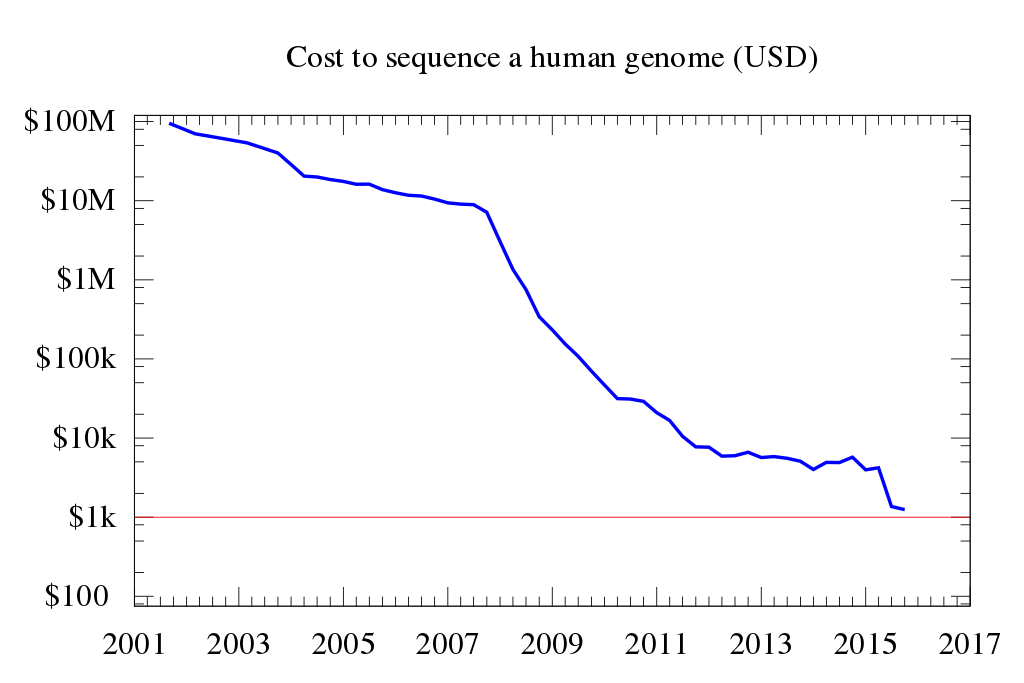
\includegraphics[width=300pt]{chapters/images/Historic_cost_of_sequencing_a_human_genome.png}
    \caption{The cost of sequencing a human-sized genome over time. Data from the NHGRI Genome Sequencing Program (GSP) }
    \label{fig:seqcost}
\end{figure}

And now we are moving into third-generation sequencing, single-molecule, long read sequencing

\newpage
\section{The bioinformatics challenge}

With huge amounts of data now being generated at relatively low cost, and compute resources being available even on moderate budgets, the challenge has shifted to development of the software able to handle these big and highly complex datasets.

Bioinformatics comes into play at various steps in the analysis process. The four main analysis tiers \cite{kulski2016next} to consider are:
\begin{enumerate}
    \itemsep-0.5em
    \item Base calling and quality scoring, typically done by software integrated into sequencing machines
    \item Mapping and/or assembling of the short reads, and variant calling
    \item Annotation, data integration, and visualisation
    \item Aggregation of heterogeneous datasets into a coherent reference data source
\end{enumerate}

Any errors or biases introduced in each of these steps can have a significant impact on downstream analyses and interpretation, and must be carefully examined in order to correct for them or assign appropriate confidence levels to results in subsequent analysis steps.

\verb+expand on each point?+

\subsection{Creating high-quality bioinformatics software}

Some concepts important to good software

\begin{enumerate}
    \itemsep-0.5em
    \item Accessibility (usability) of tools (documentation, open source, github etc, galaxy, galaxy, dependency management, docker)
    \item Reproducibility (conda, docker, galaxy, version control, code notebooks)
    \item Maintainability (testing, continuous integration, community building)
    \item Visualization (and reporting)
    \item Data management (FAIR data, LIMS, PIDs)
    \item Training
\end{enumerate}


\subsection{Accessibility}
Tools should be both easy to install and easy to use.

Most bioinformatics tools are commandline tools, and most biologists are not trained in the use of such, and even for bioinformaticians, running some of these tools can be a challenge as they are often not documented well. Just getting them installed can already be a challenge with all dependencies and OS differences

Galaxy \cite{afgan2016galaxy} provides a web interface to such tools, bringing analysis tools to the experts equipped to perfor the interpretation of the results.


\subsection*{Reproducibility}
\begin{verbatim}

- conda
- sweave/jupyter notebooks/rmarkdown/knitr


\end{verbatim}
Every lab will have had a variation of the following conversation at some point in their existence:

\textit{
\begin{itemize}
\item \textbf{Alice:} I want to redo analysis X, how was it run the last time? \\
\item \textbf{Bob:} I don't know, Charlie did it, the scripts are on their laptop \\
\item \textbf{Alice:} Who is Charlie? \\
\item \textbf{Bob:} Charlie was our PhD student, they left 6 months ago \\
\item \textbf{Alice:} How do I get this information now? \\
\item \textbf{Bob:} ... *crickets* ...
\end{itemize}
}

And this is not just a problem within a single institution; far too often, results described in journal articles are also impossible to reproduce given the information available in the manuscript. [cite the paper where they tried to reproduce nature papers]

As data analysis becomes an increasingly important part of any scientific study, it becomes more and more important to make research easily reproducible.

\subsubsection*{The Galaxy platform}




\begin{comment}
"forensic bioinformatics" -> have to figure out by trial and error what was done

https://bmcmedresmethodol.biomedcentral.com/articles/10.1186/s12874-017-0377-6

https://www.biostars.org/p/52561/

https://www.nature.com/naturejobs/science/articles/10.1038/nj7396-137a
https://www.nature.com/nm/journal/v13/n11/full/nm1107-1276b.html

\end{comment}

\subsection{Maintainability}

continuous integrations, functional testing, code review, dependency resolution (conda)

\subsection{Visualization and Reporting}

circos (maybe write the paper and include?), iFUSE, iReport

\subsection{Data Management}

\subsection{Training}
\begin{comment}can I plagiarize my own papers? :P VV\end{comment}
Rapid development of DNA sequencing technologies has made it possible for biomedical disciplines to rival the physical sciences in data production capability. The combined output of today’s sequencing instruments has already surpassed the data generation speed of resources such as the Large Hadron Collider and is rivaling those in the field of astronomy. Yet biology is different from physics (and other quantitative disciplines) in one fundamental aspect: the lack of computational and data analysis training in standard biomedical curricula. Many biomedical scientists do not possess the skills to use or even access existing analysis resources.
Such paucity of training also negatively impacts the ability of biomedical researchers to collaborate with their statistics and math counterparts, because of the inability to speak each other’s language. In addition, an estimated one-third of biomedical researchers do not have access to proper data analysis support \cite{larcombe2017elixir}. The only operative way to address these deficiencies is with training. The need for such training cannot be overstated: while the majority (>95\%) of researchers work or plan to work with large datasets, most (>65\%) possess only minimal bioinformatics skills and are not comfortable with statistical analyses \cite{larcombe2017elixir}, \cite{williams2017vision}.
This overwhelming need drives the demand, which, at present, greatly exceeds supply \cite{attwood2017global}. In a recent survey \cite{survey2013embl} over 60\% of biologists expressed a need for more training while only 5\% called for more computing power. Thus one can assume that the true bottleneck of the current data deluge is not storage or processing power, but the knowledge and skills to utilize existing resources.


\section{Importance of Analysis Software}
For each task you may wish to perform there will be a number of tools available to do the job, but which is best? Each tool will claim superiority over all the others in their publication, and all these claim are usually true, each tool can usually outperform all other under a set of hand-picked conditions.

review articles may compare several, still an optimization problem (better at subtask A but worse at subtask B)

horrible overlap (variants/SVs as example)

% choice of transcript reference
Not only the choice of software, but also the choice of reference database can hugely impact analysis results and interpretation. In variant annotation for instance, two of the most widely used transcript set reference databases are RefSeq \cite{} and ENSEMBL \cite{}, however, choosing one or the other was found to lead to wildly different variant effect predictions, with concordance as low as 44\% for putative loss-of-function variants \cite{mccarthy2014choice}.

Performing RNASeq and actually sequencing the transcripts instead of predicting will help to improve

\newpage
\thispagestyle{empty}
\begin{center}
\vspace{2cm}
\begin{minipage}{6in}
\tikz[remember picture,overlay]
\node[opacity=0.8,inner sep=0pt] at (current page.center){
    
\includegraphics[width=\paperwidth,height=\paperheight]{chapters/images/background-texture-blue.jpg}
};
\sc
\begin{center}

\color{white}{
\Large Prostate Cancer \normalsize
\vspace{2cm}


I like puzzles. Any type of puzzle. I always have. If I see a puzzle or a problem I have to solve it. I think that is what makes cancer such a fascinating topic for me.

\vspace*{0.5cm}

Imagine you are given a jigsaw puzzle. Now instead of a few hundred pieces, there are several billion pieces. The picture on the box is not a picture of the puzzle inside the box,
it is just a somewhat similar image. Oh, and did I mention there are a whole bunch of pieces missing? and that many pieces are duplicated? Some pieces don't even belong in our box,
but come from a completely different puzzle. On top of that your little sister has spilled paint over some of the pieces so those can't be trusted to contribute to the image. And instead of one
single puzzle, the box contains several, they are all variations of the image on the box, but you have no idea how many different puzzles the box contains. Sound challenging? This is the problem we are solving whenever we sequence a cancer genome.

\vspace*{0.5cm}
\textbf{[Metaphor key]} \\
\textit{puzzle pieces} = sequence reads \\
\textit{picture on box} = reference genome \\
\textit{missing pieces} = hard-to-sequence areas \\
\textit{other puzzles} = contamination \\
\textit{painted pieces} = sequencing errors \\
\textit{multiple puzzles in box} = clonality
}

\end{center}
\end{minipage}
\end{center}



\newpage
\section{Use case 1: Prostate Cancer}
\subsection{Background}
\epigraph{3in}{The time has come in America when the same kind of concentrated effort that split the atom and took man to the moon should be turned toward conquering this dread disease.}{President Richard Nixon}

On December 23, 1971, President Richard Nixon, buoyed by recent technical feats such as the moon landing, signed into law the National Cancer Act, thereby declaring a war on cancer. Today, more than 45 years later, that war is still being waged in full force. While great advancements have been made towards this goal, some of the initial optimism has been quelled by discoveries of the great complexity and heterogeneity underlying cancer.

In 2007, technological advancements enabled cancer researchers to look at the complete set of genes (the \textit{exome}) known at the time, in a set of 22 samples of 2 different tumour types. This brute-force, whole-exome sequencing (WES) method yielded a genomic landscape of \textit{mountains} of frequently mutated genes as well as a large number of \textit{hills} that were mutated at lower frequencies across patients, and highlighted once again the vast heterogeneity of cancer genomes \cite{wood2007genomic}.

Since then, many such WES studies on large cohorts of patients have been conducted \cite{wheeler2013human} and have greatly increased our insight into the mutational landscapes of the different tumor types.

...

Prostate cancer remains one of the most common cancers in men, with an estimated 1 in 7 men being diagnosed with the disease in their lifetime \cite{}[cancer.org]. Prostate tumours are often very slow growing, leading to the observation that most men die \emph{with} prostate cancer, rather than \emph{from} it. Early detection is key in selecting the optimal treatment strategy, but prostate cancer often shows few symptoms in the early stages making this a challenge.

A subset of prostate cancers (x \% [cite]) is of a more aggressive type,


\subsection{The Hallmarks of Cancer}

Tumor cells evolve from normal cells through the acquisition and accumulation of mutations. The human body has mechanisms in place to repair or dispose of damaged cells and to prevent runaway cell division, so in order for a tumour cell to survive and thrive it needs to acquire changes that provide it with advantages for proliferation and evasion of the cell's defense mechanisms. Evidence suggests this transformation from healthy cells into malignant cells follows a strikingly similar path across all different tumour types \cite{}. A cell's acquired abilities that drive tumour progression are know as the \emph{hallmarks of cancer} and consist of the following six characteristics:

\begin{itemize}
    \itemsep-0.5em
    \item self-sufficiency in growth signals
    \item insensitivity to anti-growth signals
    \item evasion of programmed cell death
    \item limitless replicative potential
    \item sustained angiogenesis
    \item tissue invasion and metastasis
\end{itemize}

Each of these steps overcomes one of the body's anti-cancer defense mechanisms. This evolution into malignancy is an almost darwinian process where the mutations acquired are random, but those cells that have gained mutations which are advantageous for survival will be able to replicate and thrive and accumulate further mutations. Distinguishing the mutations that impart a strategic advantage and thereby \emph{drive} a tumour's progression, from the often huge number of less harmful \emph{passenger} mutations accumulated over the lifetime of a cancer cell is no easy task. The optimal course of treatment for a patient often depends on the mutations present and how the cell functions are subsequently impacted by those mutations. However, many different mutations may lead to the same disruptions of key pathways, therefore we must evaluate mutations not just as the DNA level but in the broader context of their functional impact on the cell's internal processes.


\subsection{Cancer's Complexities}

Determining the exact genetic sequence of healthy individuals is already quite a challenging endeavor; trying to extend this to cancer genomes takes this challenge to the extreme. There are several complexities present in cancer geneomes that make accurate determination of the genetic changes and their downstream impacts a difficult task:

\begin{enumerate}
    \itemsep-0.5em
    \item Small variants
    \item Structural variations
    \item Clonality
    \item Temporal Evolution
    \item others? Epigenetics? transcriptome level complexities?
\end{enumerate}

In the following sections we will discuss each of these complexities and explore the biological and informatics challenges posed by them.

\subsubsection{The Bio}
\paragraph{Small variants} comprise the simplest class of mutations; those consisting of alterations of just a handful of bases, for instance the \emph{substitution}, \emph{deletion} or \emph{insertion} of one or more nucleotides.

The impact of such mutations depends on where in the genome they occur. Single nucleotide variants (SNVs) in exonic regions can range from having no effect on the resulting protein (silent) to changing an amino acid in the protein to a different amino acid (missense mutations), to changing a codon into a stop codon (nonsense mutation) which nearly always results in a nonfunctional protein. If this happens in a protein that is vital to the functioning of the cell this can have disastrous consequences <some examples of SNVs causing serious problems/phenotypes> <conserved regions, cell's mechanisms for preventing such fatal flaws>

These simple variations were the first to be extensively studied and found to contribute ..

While variants within the coding sequence are most likely to have an impact on cell health, small variants \emph{outside} the coding sequence can also have drastic impact on health, for example 70\% of melanomas exhibit a point mutation in one of two positions in the promoter region of TERT (Horn et al. 2013; Huang et al. 2013).

\paragraph{Structural variations} are larger-scale mutations, involving rearrangement of segments of DNA of more than roughly 50 bp. These often do not involve the coding sequences directly, and can therefore only observed through whole-genome sequencing.

<fusion genes>


\paragraph{Clonality}
\paragraph{Temporal Evolution}
\paragraph{Epigenetics}

\subsubsection{The Informatics}

We know that changes in sequence and structure of DNA contributes to cancer development. But how do we describe these properties? Any two healthy individuals differ greatly in their DNA sequence; it's what makes us us. How to denote these differences is a non-trivial problem, as is determining which of these differences are just part of the natural variation between individuals and which are ones detrimental to our health and functioning.

If you were asked to describe the differences between two Shakespeare plays, how would you go about it? They are made up of the same alphabet, and share many of the same words and even whole sentences, but to list the differences between them can be done in many ways. You could number the words in both books and take note of the ones that are different in each position, but then if you were to take two identical sentences and prefix one with a single extra word, all positions would end up being flagged as different while clearly these sentences are nearly identical. And ..

<note: ditch the book analogy? example shakespearean sentence to illustrate? >

poor concordance between variant callers: https://genomemedicine.biomedcentral.com/articles/10.1186/gm432


Currently variations in DNA are described relative to a \emph{reference genome}; a sequence intended to represent the \emph{average} human genome, which was constructed by taking the most frequently observed nucleotide at any given  position in the genome
<discuss some drawbacks/things to realize: based on relatively small set of samples, not optimally diverse set of individuals>

As we have seen, the choice of software can impact downstream analysis, and variant calling is no exception. Different aligners employ different mapping strategies, which leads to different variant calls for the same observed sequence depending on the choice of algorithm, complicating variant comparisons between studies \cite{zook2014integrating}. While there do exist tools to canonicalise some of these differing representations \cite{vcflib}, complex variants remain that do not have a single obvious standard form (Figure \ref{fig:variant-multiple-representations}).
But even for the simpler cases, there is not always a clear consensus on how to standardise representation. Consider for instance the case where an adenine nucleotide has been inserted, transforming the sequence \verb+TAAG+ to \verb+TAAAG+. Do we describe the insertion to have happened at position 1 (after the \verb+T+), position 2 (between the two \verb+A+s), or at position 3 (before the \verb+G+)? While this particular case is easily solved by agreeing on a convention of either left-aligning or right-aligning these variants, such community agreement does not currently exist, with most next-generation analysis tools opting for left-alignment, while certain variant databases such as HGVS [TODO cite] still recommend (but do not enforce) alignment to the position nearest the 3\` end of the gene \cite{hgvs-position}, which translates to right-alignment in genomic coordinates for reverse strand genes. Furthermore, once variants have been submitted to online databases, information about surrounding variants observed in the same sample is often not kept, making it impossible to resolve equivalency of variant representations going forward.

\begin{figure}[h!]
    \centering
    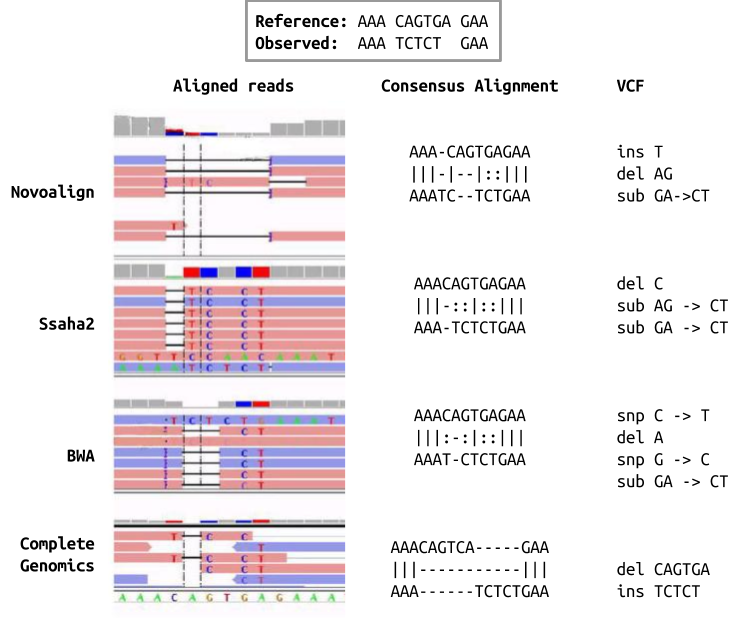
\includegraphics[width=400pt]{chapters/images/variant-representation-all.png}
    \begin{comment}
        image in google drive https://docs.google.com/drawings/d/1WWmzW6uWtJ7HZ5WVgtg_oAMA_3E_569M4Ikjz4Ecjic/edit
    \end{comment}
    \caption{Complex variants can be represented in multiple ways. Four different aligners (Novoalign, Ssaha2, BWA, Complete Genomics) treat the same variant in vastly different ways, which leads to such differing sets of variant descriptions in the VCF files that it is no longer apparent that these variants in fact describe the same observed sequence.}
    \label{fig:variant-multiple-representations}
\end{figure}


<not to mention sequencing errors, at rate of abt x/100, sequencing depth helps but tradeoff with cost>

sources of mismatch with reference genome \\
- real mutation \\
- wrong base call \\
- wrong mapping/variant call \\


<repetitive regions>

The result of all of this is that different variant calling tools will produce different sets of variants given the exact same input dataset and reference genome, and it is hard to know who does a better job, if their respective papers are to be believed each one of them far outstrips all the others. But as with everything in life, the truth lies somewhere in the middle. Each of the variant callers has its strengths and weaknesses, some may very accurate in calling one type of variant but have  more difficulty with others. Some are very accurate in healthy genomes but less so in highly mutated genomes or vice versa. One possible solution is to run a set of variant callers

\paragraph{Structural variations}
<very very poor overlap between different methods>

<hard to resolve exact location of junctions>

<chainfinder>
\paragraph{Clonality}
\paragraph{Temporal Evolution}
\paragraph{Epigenetics}



\newpage
\thispagestyle{empty}
\begin{center}
\vspace{2cm}
\begin{minipage}{5in}
\tikz[remember picture,overlay]
\node[opacity=0.8,inner sep=0pt] at (current page.center){
    
\includegraphics[width=\paperwidth,height=\paperheight]{chapters/images/background-texture-blue.jpg}
};
\sc
\begin{center}

\color{white}{
\Large Metagenomics \normalsize
\vspace{2cm}

blabla

\vspace*{0.5cm}

}

\end{center}
\end{minipage}
\end{center}

\newpage


\section{Use case 2: Microbiota}


\subsection{The Bio}
first complete bacterial genomes published in 1995  \cite{land2015insights}

16S rRNA

whole genome shotgun

\subsection{The Informatics}


\begin{comment}
history of microbiolgy: https://courses.lumenlearning.com/boundless-microbiology/chapter/introduction-to-microbiology/

<WGS reveals changes outside coding regions, such as one affecting regulation of genes are of importance, and can reveal large scale changes (SVs), fusion genes>

<epigenetics>

<potential of developing treatments from all this knowledge>

sources:
- Hallmarks of cancer: the next generation [@hanahan2011hallmarks]
- Chromosome aberrations in solid tumors [@albertson2003chromosome]

~~~
low-resolution methods:
- fluorescent in sit hybridisation FISH [Pinkel et al 1988, Thompon and Gray, 1993]
- chromosome painting [Jauch et al, 1992]
- spectral karyotyping [Schrock et al 1996]
- comparative genome hybridisation CGH [Kallioneimi 1992]

- arrays

high-throughput:
 - LOH [@hampton1996simultaneous]
 - GWAS

 - 2003 still infeasible to sequence entire tumor genome, so
   ESP (end sequencing profiling) used [Volik et al 2003]
       (- BAC library from tumor, sequence ends, map to reference)
    → reconstruction from ESP data [Rapael et al 2003]

now: WGS
- NGS: DNA short reads
- NGS: RNA Seq
- NGS: Paired end mapping [@korbel2007paired]
- limitations of current methods
~~~

advanced in cancer research specifically from next generation methods: [@meyerson2010advances]

\end{comment}







\begin{comment}

types of SVs: standard, complex, chromothripsis [@stephens2011massive]

- well-known examples
    - TMPRSS ERG
    - ABL gene on chr9, chronic myeloid leukema, translocation between chr9 and 22,
       changes regulation, promotor becomes promotor of BCR gene on chr22
      [Heisterkamp et al 1983]

#### usefulness in biomarker and treatment development

- Gleevec, targeting BCR-ABL fusion gene [@druker2001efficacy]
- Herceptin, targeting ERBB2 amplification [@kauraniemi2004effects]


#### SV Tools and databases

~~~
- catalogued in Mitleman database [Mitelman 2003]
- COSMIC
- ..
~~~

## Clonality

## Temporal evolution

## etc..
~~~
<Informatics/analysis methods>
 - History of methodologies (gwas, ..)
 - NGS: Huge datasets, excel and manual analyses no longer suffice
 - Cancer: Germline correction, drivers vs passengers

<Limitations of current methods>
 - imperfect data
 - disagreements and biases per lab/informatics technique

<Challenges in tumour genome reconstruction>
→ explain in biology section, here describe why that complicates things

 - Normal Contamination
 - Clonality detection
 - Event Chains detection
 - Temporal evolution detection


\end{comment}


\bibliographystyle{plain}
\bibliography{references}
